% Chapter 4
%http://www.cs.iit.edu/~oaldawud/CS487/project/software_design_specification.htm


\chapter{Architecture of the Engine}
%\epigraph{A fancy quote.}{Me}

\label{engine} % For referencing the chapter elsewhere, use \ref{Chapter2} 

\lhead{Chapter 4. \emph{Architecture of the Engine}} % This is for the header on each page - perhaps a shortened title

This chapter describes the architecture of a possile timetabling engine. It describes internal data structures, a data model and a possibility for a timetabling algorithm. Other important topics like the evaluation function and computational complexity are also discussed.

\section{Data design}
Data design is an important step in software development. It is a process that gives a good overview of how the data will be organized and accessed. Characteristics like simplicity, fast data access, extensibility and maintainability were kept in mind when designing such structures.    
\subsection{Solution Representation}


Usually, in a formal definition of the University Class Timetabling Problem, we have a set of \textit{n} events, a set of \textit{m} rooms and a set of \textit{t} available time slots. This means that we have \textit{m} $\cdot$  \textit{t} possible places where to schedule the events and it is easy to see that the problem is only solvable if \textit{m} $\cdot$  \textit{t} $\geq$ \textit{n} .\\
Since we know that we cannot have two different events with same combination of a room and a time slot, a possible representation for a timetable is a  matrix in which rows represent the rooms and the columns represent the time slots. Besides, this representation does not allow the scheduling of different events in the same room, and thus solves an important constraint and reduces drastically the search space. This brings an advantage against other possible representation that do not take this fact into account, for example, an array of size \textit{n} where each cell indexes a time slot and a room. In fact, if we did not consider this information and that each event occurs in a single time slot, the total number of ways of assigning \textit{n} events to \textit{m} $\cdot$ \textit{t} places would be:

\begin{center}
$(m \cdot t)^{n}$
\end{center}

On the other hand, this representation reduces search space to:
\begin{equation}
\label{comb_assign}
\begin{split}
\binom{m \cdot t}{n} \cdot n! & = \frac{(m \cdot t)!}{n! (m \cdot t - n)!} \cdot n! \\
& = \frac{(m \cdot t)!}{(m \cdot t - n)!}
\end{split}
\end{equation}

In Eq. \ref{comb_assign}, the first factor represents the arrangement of these $n$ events over the \textit{m} $\cdot$ \textit{t} places and the second factor of the first member represents the possible permutations of an assignment.
Figure \ref{fig:solution_representation} shows a very simple scenario with 2 week days (represented by different colors), 10 events and 10 rooms. Each cell has the id of the scheduled event and may have only one. Besides, there may be events of longer duration occupying more than one cell.

\begin{figure}[t]
	\centering
	\resizebox{\textwidth}{!}{
	    \input{./Figures/tkiz/solution.tkiz} 
	  }
	\rule{35em}{0.5pt}
	\caption[Solution representation]{Solution representation} 

	\label{fig:solution_representation}
\end{figure}

In order to restrict the search space even more, we use additional information mainly regarding constraints and availabilities. 
}
Figure \ref{fig:search_space} shows a representation of the search space for this problem. The green areas represent the feasible solutions and the red areas represent solutions that are forbidden (unfeasible) because of additional constraints.

\begin{figure}[t]
	\centering
	    \input{./Figures/tkiz/search_space.tkiz} 
		\rule{35em}{0.5pt}
	\caption[Search Space]{Search Space} 
	\label{fig:search_space}
\end{figure}


\subsection{Data Structures}

In order to maintain information regarding constraints some auxiliary data structures may be used. Besides, additional data regarding the current state of the solution may also be  kept in memory because it helps to speed up constraint violations checks. In this section, we introduce the data structures used and in the next section we make a comprehensive review of the operations that make use of these structures and also a time and space complexity analysis. \\
Usually, precedences happen between events lectured by the same teacher(s). Thus, it is useful to keep in memory information regarding the current order of assigned events for each teacher. Figure \ref{fig:teacher_events_timeslots} shows a possible representation of this information. The head nodes store the teachers ids and the lists store the event ids. For example, in Figure \ref{fig:teacher_events_timeslots} there are five teachers and for instance the first teacher has the events 2 and 5 assigned.
Figure \ref{fig:precedence_matrix} shows a matrix that stores information about precedences between events. Precedences may be hard or soft, for example, a theory lecture event must happen before a practical event but between practical events, this constraint may be soft. Each  cell with 1 represents a hard precedence, whereas 2 represents soft precedences between events. 

\begin{figure}[th]
	\centering
	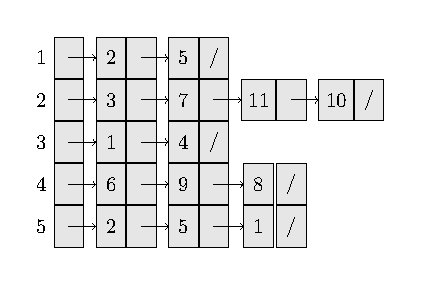
\includegraphics[scale=0.95]{./Figures/tkiz/teacher_schedule.pdf}
	\rule{35em}{0.5pt}
	\caption[Current order of teacher events]{Current order of teacher events} 
	\label{fig:teacher_events_timeslots}
\end{figure}
\

 Figure \ref{fig:distance_matrix} shows a distance matrix where each cell represents the minimum required temporal distance between two events. For example, in Figure \ref{fig:distance_matrix} the events 3 and 5 should have a temporal distance of 5 time slots. In order to quickly check if the distance between two events is being respected, an associative array that stores the beginning time slot of each event is useful because one only needs to compute the distance between two events and compare it with the information in the distance matrix. Each index represents a single event and maps the first time slot at which an event begins.\\

\begin{figure}[thp] 
  \label{ fig7} 
  \begin{minipage}[b]{0.5\linewidth}
		\centering
		\input{./Figures/tkiz/precedences.tkiz}
		\caption[Precedence matrix]{Precedence matrix}
		\label{fig:precedence_matrix}
		\vspace{4ex}
  \end{minipage}%%
  \begin{minipage}[b]{0.5\linewidth}
        \centering
        \input{./Figures/tkiz/distances.tkiz}
		\caption[Distance matrix]{Distance matrix}
		\label{fig:distance_matrix}
    \vspace{4ex}
  \end{minipage} 
  \begin{minipage}[b]{0.5\linewidth}
	    \centering
		\input{./Figures/tkiz/restrictions.tkiz}
		\caption[Constraint matrix]{Constraint matrix}
		\label{fig:constraint_matrix}
		\vspace{4ex}
  \end{minipage}%% 
  \begin{minipage}[b]{0.5\linewidth}
        \centering
		\input{./Figures/tkiz/pa.tkiz}
		\caption[Teacher availability]{Teacher availability}
		\label{fig:teacher_matrix}
    \vspace{4ex}
  \end{minipage} 
    \begin{minipage}[b]{0.5\linewidth}
        \centering
		\input{./Figures/tkiz/ra.tkiz}
		\caption[Room availability]{Room availability}
		\label{fig:timeslot_room_matrix}
    \vspace{4ex}
  \end{minipage} 
   \begin{minipage}[b]{0.5\linewidth}
        \centering
		\input{./Figures/tkiz/ru.tkiz}
		\caption[Room usage]{Room usage}
		\label{fig:room_usage}
    \vspace{4ex}
  \end{minipage} 
\end{figure}

Figure \ref{fig:constraint_matrix} represents multiple constraints encoded in a single matrix. One for contiguous events, two for events occurring in different days, three for events occurring in different time slots, four for overlapped events, five for events starting at the same time and finally six for events occurring in the same day. Once again, an associative array is useful because it allows to quickly locate the events and then perform small computation checks.\\
Figure \ref {fig:teacher_matrix} shows a matrix with the teacher availabilities encoded. This matrix serves only for fast availability checks. Essentially, a teacher may be available in a time slot (0) or recently unavailable (1), i.e, during the search, this value may become 0 again. It is important to note that this matrix translates the actual state of the teacher availabilities according to the current solution, that is, the current teacher availability that may change in the future. This matrix is useful when trying to place a teacher in a time slot. The teacher will only be placed if this matrix allows it (value 0 in the corresponding time slot). It is important to remember that each teacher has an ordered list of preferential time slots and it is represented with a similar structure shown in Figure \ref{fig:teacher_events_timeslots}. In this case, the lists contain time slots. The search starts in this list, and for each preferential slot, it checks the matrix and thus avoiding an important restriction of not placing teachers in non desired time slots and in unavailable time slots.\\
As explained in the Chapter \ref{current_process}, there is an order in which the departments create the schedules. Therefore, it is natural that certain rooms are always unavailable in certain time slots (because they have scheduled lectures from another department). In order to take into account this information, the matrix represented in Figure \ref{fig:timeslot_room_matrix} may be used. Similar to the teacher availabilities, zero values represent available time slots and cells with the number one represent unavailable time slots. The structure presented in Figure \ref{fig:room_usage} is useful to measure the room usage. Each time an event is inserted in the time table, the value of the cell is incremented (different events may belong to the same subject). The final value for each subject or teacher (in the last row) is the number of rooms currently in use. For example, in Figure \ref{fig:room_usage} the teacher with the id 7 is currently using 2 different rooms (2 times in the room 5 and one in room 6). On the other hand, the same kind of structure (but in a different matrix) may also encode the room usage by subjects, following the same idea.

\begin{figure}[t]
	\centering
	    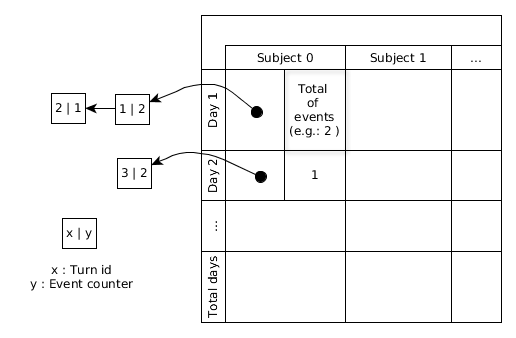
\includegraphics[scale=0.45]{./Figures/DataStructures/yED/cp_tracking_distribution.png}
	\rule{35em}{0.5pt}
	\caption[Structure to keep track of the distribution of events]{Structure to keep track of the distribution of events} 
	\label{fig:distribution_events}
\end{figure}

Figure \ref{fig:distribution_events} represents a structure useful to count the distribution of a subject over the week. For each day and for each subject, each time an event is inserted, the corresponding node is incremented. Therefore, each node counts the number of events from a given turn from a certain subject in a certain day, simulating the point of view of a student who attends classes from that turn. With this structure updated, it is easy to compute the distribution of events (number of days) from a subject (from the point of view of the student). One only needs to check how many days with non zero values exist (for each subject), represented in the example by the final row. For instance, in Figure \ref{fig:distribution_events}, in the first day, the subject with id 0 is having classes from turn 1 and 2, and classes from turn 3 in the second day.\\

\begin{figure}[h]
	\centering
	    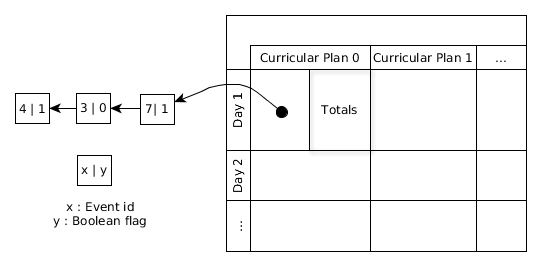
\includegraphics[scale=0.45]{./Figures/DataStructures/yED/cp_tracking.png}
	\rule{35em}{0.5pt}
\caption[Generic structure to keep track of events]{Generic structure to keep track of events} 
	\label{fig:tracking_cp_events}
\end{figure}

In order avoid full table scans, there is the need to maintain a generic structure that keeps track of the events of each curricular plan, in each day is useful. Figure \ref{fig:tracking_cp_events} shows a simple example of this structure. Besides it is also useful to store additional information about the current state of the solution. In the example, for each cell in the matrix there is a sorted list of events happening on that day. There is also information that may be extracted from that current list and is stored as a list of values represented in the Figure \ref{fig:tracking_cp_events} by totals. These totals are important when analyzing constraints because they give immediate feedback that is useful to decide if certain constraints are met. Another important aspect of this structure is that avoids double countings, i.e, if certain constraints do not consider the differences between events from the same class and typology, it is important to also keep track of which events are already considered. In Figure \ref{fig:tracking_cp_events} each element from the list contains the event id and if it is already counted or not. Further explanation about this structure is explained in the next section where an analysis of the complexity of the operations is made. 

\begin{figure}[t]
	\centering
	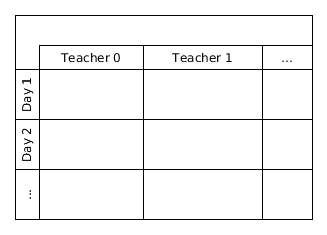
\includegraphics[scale=0.5]{./Figures/DataStructures/yED/generic_info_tracking.png}
	\rule{35em}{0.5pt}
	\caption[Generic structure to store numerical data about teachers]{Generic structure to store numerical data about teachers} 
	\label{fig:teacher_stats_track}
\end{figure}

Another useful structure to keep information about teacher is a matrix presented in Figure \ref{fig:teacher_stats_track}. Each cell of this matrix stores numerical data that changes over time and reflects some aspects from the current solution.

\section{Complexity and Performance Issues}

One of the main operations of the timetabling algorithms is to check constraint violations. Therefore, it is important to these validations to be reasonable fast, i.e, it should be avoided scanning the entire timetable when making the decision if a certain solution is feasible or not. The key idea is to increase the speed of the validations at the cost of using more memory.
\label{lab:complexity_analysis}

\begin{table}[H]
\centering
\begin{tabular}{|l|c|c|}
\hline
	Operation & Worst-Case Analysis \\
\hline
	Array lookup & $\mathcal{O}(1)$ \\
	\hline
	Matrix lookup & $\mathcal{O}(1)$ \\
	\hline
	Precedences/Distance/Constraint matrix scan & $\mathcal{O}(E^2)$ \\
	\hline
	Insert teacher event (Figure \ref{fig:teacher_events_timeslots}) & $\mathcal{O}(E)$ \\
	\hline
	Delete teacher event (Figure \ref{fig:teacher_events_timeslots}) & $\mathcal{O}(E)$ \\
	\hline
	Insert event (Figure \ref{fig:tracking_cp_events}) & $\mathcal{O}(E)$ \\
	\hline
	Delete event (Figure \ref{fig:tracking_cp_events})& $\mathcal{O}(E)$\\
\hline
\end{tabular}
\caption[Time-complexity of various operations]{Time-complexity of various operations\\ \textit{E} - Number of events}
\label{tab:complexity_operations}
\end{table}

Table \ref{tab:complexity_operations} shows the worst-case complexity of some common operations that are performed when analyzing constraints. In order to insert events in the structure presented in Figure \ref{fig:tracking_cp_events} an initial scan is needed to correctly set the flag. Then a second scan is performed to insert the new event in the correct order. On the other hand, when deleting an event, if the event was previously set with the flag 1 (meaning that this event was being counted), another event must be chosen (from the same subject) and set with a new positive flag. This involves, at most, two complete scans on this list.

Table \ref{tab:new_common_constraints} shows a set of flexible constraints, i.e., they may be considered hard or soft constraints. These constraints are essentially the same as the constraints used by the Bullet Solutions software.
It is also shown the worst case complexity for each case. The first presented complexity is applicable when a solution is being analyzed considering all of the events, i.e, the entire solution. The second is applicable to the computation of the difference between an old solution and a new one, i.e, an incremental approach where every time a new event is inserted, only the potential changes to the solution are computed and updated. This allows the solution to be always feasible because forbids invalid moves.   
\begin{table}[H]
\centering
\resizebox{\textwidth}{!}{%
\begin{tabular}{|p{10cm}|c|c|c|c|}
\hline
\multicolumn{1}{|c|}{\multirow{2}{*}{Hard / Soft Constraint}} & \multicolumn{2}{|c|}{Worst-Case Analysis } \\
\cline{2-3}   & Entire Solution & Incremental Approach\\
\hline
	Order of typologies must/should be respected (Figure \ref{fig:precedence_matrix}) & $\mathcal{O}(P \cdot E)$  & $\mathcal{O}(E)$\\
\hline
	Event A and B must/should be contiguous  (Figure \ref{fig:constraint_matrix}) & $\mathcal{O}(E^2)$ & $\mathcal{O}(E)$\\
\hline
	Event A and B must/should be overlapped (Figure \ref{fig:constraint_matrix}) &  $\mathcal{O}(E^2)$ & $\mathcal{O}(E)$ \\
\hline
	Event A and B must/should not be overlapped (Figure \ref{fig:constraint_matrix}) & $\mathcal{O}(E^2)$ & $\mathcal{O}(E)$\\
\hline
	Event A and B must/should be in different days (Figure \ref{fig:constraint_matrix}) & $\mathcal{O}(E^2)$ & $\mathcal{O}(E)$\\
\hline
	Event A and B must/should start at the same hour & $\mathcal{O}(E^2)$ & $\mathcal{O}(E)$\\
\hline
	Event A and B must/should be in the same day & $\mathcal{O}(E^2)$ & $\mathcal{O}(E)$\\
\hline
\end{tabular}%
}
\caption[Complexity of common (hard/soft) constraints used in the engine]{Complexity of common(hard/soft) constraints used in the engine.\\ \textit{P} - Number of teachers, \textit{E} - Number of events}
\label{tab:new_common_constraints}
\end{table}

In order to check if precedences are being respected, one only has to look at the current events order of a teacher. This order is stored in a structure like the one presented in Figure \ref{fig:teacher_events_timeslots}. An additional look up at the associative array (in order to obtain the beginning time slot of each event) is needed, which is a constant operation. The remaining constraints presented in Table \ref{tab:new_common_constraints} are translated into two simple lookups (per two events) to the associative array of events and the afterwards computation.\\


Table \ref{tab:new_hard_constraints} shows the hard constraints considered and their worst-case complexity. It is important to note that some constraints are excluded by definition, i.e, they are solved thanks to the chosen representations, for instance, two different events must not share the same
room and time slot or the fact that teachers are not scheduled in unavailable time slots. 
 

\begin{table}[H]
\centering
\resizebox{\textwidth}{!}{%
\begin{tabular}{|c|p{8cm}|c|c|c|c|}
\hline
	\multicolumn{1}{|c|}{\multirow{2}{*}{Point of View}} & \multicolumn{1}{|c|}{\multirow{2}{*}{Hard Constraint}} & \multicolumn{2}{|c|}{Worst-Case Analysis } \\
 &  &  Entire Solution & Incremental Approach\\
\hline
	Event & All distances between events must be respected (Figure \ref{fig:distance_matrix}) & $\mathcal{O}(E^2)$& $\mathcal{O}(E)$\\
\hline
	Student & Lunch hours for each curricular plan should be respected & $\mathcal{O}(E^2)$ & $\mathcal{O}(1)$  \\
\hline
	Student & A student cannot attend two obligatory subjects from the same curricular plan at the same time & $\mathcal{O}(E^2)$ & $\mathcal{O}(E)$ \\
\hline
	Teacher & A teacher must not be scheduled in two time slots at the same time (Figure \ref{fig:teacher_events_timeslots})& $\mathcal{O}(P\cdot E)$ & $\mathcal{O}(E)$ \\
\hline
	Teacher  & Lunch hours must be respected (Figure \ref{fig:teacher_events_timeslots}) & $\mathcal{O}(P \cdot E)$ & $\mathcal{O}(1)$ \\
\hline
	Teacher & Maximum number of hours per day must be respected (Figure \ref{fig:teacher_stats_track}) & $\mathcal{O}(P \cdot D)$ & $\mathcal{O}(1)$\\
\hline
	Teacher & Maximum number of consecutive hours per day must be respected (Figures \ref{fig:teacher_events_timeslots},\ref{fig:teacher_matrix}) & $\mathcal{O}(P \cdot E)$ & $\mathcal{O}(T)$\\
\hline
	Student & Maximum number of hours per day for each curricular plan must be respected (Figure \ref{fig:tracking_cp_events}) & $\mathcal{O}(D \cdot PC)$ & $\mathcal{O}(1)$\\
\hline
	Student  & Maximum number of consecutive hours per day for each curricular plan must be respected  (Figure \ref{fig:tracking_cp_events}) & $\mathcal{O}(D \cdot PC)$ & $\mathcal{O}(E)$\\
\hline
	Classroom  & A room cannot be scheduled in unavailable time slots (Figure \ref{fig:timeslot_room_matrix}) & $\mathcal{O}(E)$ & $\mathcal{O}(1)$  \\
\hline
\end{tabular}%
}
\caption[Complexity of hard constraints used in the engine]{Complexity of hard constraints used in the engine\\\textit{P} - Number of teachers, \textit{E} - Number of events, \textit{D} - Number of days, \textit{T} - Number of time slots, \textit{PC} - Number of Curricular Plans}
\label{tab:new_hard_constraints}
\end{table}


In order to check if the distances between the events are being respected, the distance matrix has to be completely scanned and for each pair of events, two lookups to associative array are made. If only the inserted event is considered, then only one dimension of the distance matrix is scanned.\\
Each curricular plan may have a lunch hour. This is solved by checking the time slots where the events are, by using the associative array, and comparing against a structure that stores lunch hours for each curricular plan. When inserting a event, a simple lookup to this matrix with lunch hours is enough to decide. \\
To verify that a teacher does not have two different events in the same time slot, the structure presented in Figure \ref{fig:teacher_events_timeslots} is useful because one only needs to check that there are not two events in the same list share the same time slot. An additional lookup to the associative array is needed to obtain the starting time. \\
A teacher has a list of preferential time slots associated, i.e, the unavailable time slots are not in this list. Therefore, we can always guarantee that a teacher will be placed in a time slot available to him. This situation is similar to the classrooms because there is a matrix that stores the unavailabilities. Simple lookups to this matrix solves the constraint. \\
The matrix presented in Figure \ref{fig:teacher_stats_track} may store information about the current total of hours that a teacher is having per day. With this structure updated, it is very easy to check if an event may be inserted in a certain time slot or how many teachers are currently with too much hours (assuming that each event insertion updates this matrix). On the other hand, each time an event is inserted, the current teacher availability matrix is useful to quickly compute how many consecutive hours that insertion will cause. One only needs to count the consecutive positive values before that time slot and compare it with the allowed maximum. The alternative is to scan the events of each teacher and compute the current maximum consecutive hours, with the aid of some lookups in the associative array.\\
Each curricular plan must have a limit of hours per day. In this case the structure presented in Figure \ref{fig:tracking_cp_events} is useful to store this data for each curricular plan and for each day. This value is one of the totals that may be stored and reflects the currently total of hours present in the corresponding list of events. It is important to note that different events belonging to the same subject and typology but with different turns must be counted as one (a student only attends one) and this implies that when a new event is inserted to this list, it must be set with the correct flag (0 - Do not count this event, 1 - Count this event). The insert operation involves a scan to this list in order to set the correct flag and another scan in order to place the event in the correct order. This sorted listed is also used to compute current maximum number of consecutive hours and it is achieved with a simple scan to this list.

Table \ref{tab:new_soft_constraints} shows the soft constraints and their worst case complexities.						

\begin{table}[H]
\centering
\resizebox{\textwidth}{!}{%
\begin{tabular}{|p{0.5cm}|p{7cm}|c|c|c|c|}
\hline
	\multicolumn{1}{|c|}{\multirow{2}{*}{Point of View}} & \multicolumn{1}{|c|}{\multirow{2}{*}{Soft Constraint}} & \multicolumn{2}{|c|}{Worst-Case Analysis } \\
 &  &  Entire Solution & Incremental Approach\\
\hline
	Student & Events of a subject should be distributed over a minimum number of days (Figure \ref{fig:distribution_events})& $\mathcal{O}(S \cdot D)$ & $\mathcal{O}(U)$\\
\hline
	Student & For each curricular plan, the number of holes between events should be minimized (Figure \ref{fig:tracking_cp_events}) & $\mathcal{O}(D \cdot PC)$ & $\mathcal{O}(E)$\\
\hline
	Student & The number of rooms used by a subject should be minimized (Figure \ref{fig:room_usage}) & $\mathcal{O}(R \cdot S)$ & $\mathcal{O}(R)$\\
\hline
	Student & For each curricular plan, the minimum number of hours per day should be respected (Figure \ref{fig:tracking_cp_events}) & $\mathcal{O}(D \cdot PC)$ & $\mathcal{O}(E)$\\
\hline
	Student & Events in the last slot of the day should be avoided (Figure \ref{fig:tracking_cp_events}) & $\mathcal{O}(D \cdot PC)$ & $\mathcal{O}(E)$\\
\hline
	Student  & Days with only one event should be avoided (Figure \ref{fig:tracking_cp_events}) & $\mathcal{O}(D \cdot PC)$ & $\mathcal{O}(E)$\\
\hline
	Student  & Each day should have a number of free periods (Figure \ref{fig:tracking_cp_events}) & $\mathcal{O}(D \cdot PC)$ & $\mathcal{O}(E)$\\
\hline
	Student & Each day should have events of different typologies assigned (Figure \ref{fig:tracking_cp_events}) & $\mathcal{O}(D \cdot PC)$ & $\mathcal{O}(E)$\\
\hline
	Student & Optional and obligatory subjects should not overlap & $\mathcal{O}(E^2)$ & $\mathcal{O}(E)$\\
\hline

	Teacher & The number of holes between events should be minimized (Figure \ref{fig:teacher_events_timeslots}) & $\mathcal{O}(P\cdot E)$ & $\mathcal{O}(E)$\\
\hline
	Teacher & The number of rooms used by a teacher should be minimized (Figure \ref{fig:room_usage}) & $\mathcal{O}(R \cdot P)$ & $\mathcal{O}(R)$\\
\hline
	Teacher & The minimum number of hours per day should be respected (Figure \ref{fig:teacher_stats_track}) & $\mathcal{O}(P \cdot D)$ & $\mathcal{O}(1)$\\
\hline

	Teacher & Each day should have a number of free periods (Figure \ref{fig:teacher_events_timeslots}) & $\mathcal{O}(P\cdot E)$ & $\mathcal{O}(E)$\\
\hline
\end{tabular}%
}
\caption[Complexity of soft constraints used in the engine]{Complexity of soft constraints used in the engine\\\textit{P} - Number of teachers, \textit{E} - Number of events, \textit{D} - Number of days, \textit{T} - Number of time slots, \textit{PC} - Number of curricular plans, \textit{S} - Number of Subjects, \textit{R} - Number of rooms, \textit{U} - Number of turns of a given subject}
\label{tab:new_soft_constraints}
\end{table}

In order to check the distribution of events of the subjects, the structure presented in Figure \ref{fig:distribution_events} has to be transversed in order to compute the total of days for each subject. Besides, each time an event is inserted, the corresponding total is updated, which implies transversing only the corresponding list of events in the structure.\\
For each curricular plan, the number of holes in each day may be counted by scanning the sorted list of events (Figure \ref{fig:tracking_cp_events}), i.e, counting how many times two events (from different typologies) do not overlap. This constraint conflicts with the one that states a maximum number of consecutive hours, so there is a trade off here.  
Using the structure presented in Figure \ref{fig:room_usage}, it is easy to check the room usage by scanning this matrix.  Counters that may be stored in the structure presented in Figure \ref{fig:tracking_cp_events} are the number of events in the last slot of the day, the number of events currently happening in each day, the number of free periods in each day and the number of events with different typologies in each day. These values are again obtained by scanning the list of events from each day and curricular plan. Additional lookups to the associative array table are also needed.\\
Sometimes it's desirable that obligatory subjects and optional do not overlap. This gives students the opportunity to attend both. This special case happens when there are more than one possible branch in the curricular plan. Thus, the number of overlapping events in this case should be minimal in order to let students attend some optional subjects from another curricular plan.   
The number of holes and free periods in the teacher schedules can be measured using the structure presented in Figure \ref{fig:teacher_events_timeslots}. The structure in Figure \ref{fig:teacher_stats_track} is used to get the number of hours per day and the structure like the one presented in Figure \ref{fig:room_usage} may also be used to scan the number of rooms currently in use by a teacher. 




\section{Evaluation Function}
The role of the evaluation function is to measure the quality of any solution. It plays an important role when trying to optimize a problem. The main objective in this problem is to maximize it, i.e, minimize the number of constraint violations.\\
Since hard constraints cannot be violated, the evaluation function only needs to focus on the violation of soft constraints. Soft constraints may be violated at the cost of contributing a penalty to the objective function. Besides, we can assign a weight to each violated constraint. The weights reflect the relative importance of each constraint. Eq. \ref{cost_function} shows how the value of the objective function of any solution can be computed.

\begin{equation}
\label{cost_function}
\begin{split}
	f(s) &= \sum_{i=1}^{SC} w_i(s) \cdot C_i(s) \\
\end{split}
\end{equation}

In Eq. \ref{cost_function}, \textit{s} represents a solution in the search space. The value \textit{C$_i$} represents the number of times that the constraint is violated by the solution \textit{s}, \textit{w$_i$} represents the respective weight and \textit{SC} represents the number of soft constraints. The objective of the search algorithm will be to find a solution \textit{s} that minimizes the value of \textit{f(s)}.

\section{Timetabling Algorithm}

There are many possible techniques to approach the timetabling problem. In this section we discuss a possible example based on a two-stage approach, i.e, it first tries to achieve a feasible timetable where all the hard constraints are solved and only then tries to optimize the current solution through local search techniques. This approach can then be divided into two main phases called a constructive phase where an initial solution is built and then a optimization phase where a high quality solution is sought.

\subsection{Example of a Constructive Heuristic}

In order to build an initial feasible solution, a simple sequential assignment is followed. It is important to note that this assignment is not complete deterministic, i.e, for repeated executions from the same input it may give different results. This is important because one may want to halt the program and restart the procedure, or the procedure may get in a situation where it cannot place an event in a feasible place after many iterations. Thus, it is desirable that the mechanism has some degree of randomness. Algorithm~\ref{alg:constructive_heuristic} shows the algorithm for constructing an initial solution:

\begin{algorithm}[t]
\begin{algorithmic}
\Require List of unassigned events, incomplete timetable, maximum number of iterations without successful placement 
\While{there are unassigned events}

\If{$i\geq maxIterations$}
	\State\hspace{\algorithmicindent} \Call{restartProcess}{}
\Else
	\State $e\gets $ choose an unassigned event
	\State $np\gets $ get number of feasible places for the event $e$\\
	\If{$np \geq 1$}
		\State $t,r \gets $ choose a time slot and a room for event $e$
		\State place event $e$ in time slot $t$ and room $r$
		\State remove event from the list of unassigned events
		\State $i\gets 0$
	\Else
		\State move events within the timetable
		 \State $i\gets i+1$
	\EndIf
\EndIf
\EndWhile

\caption{Constructive Heuristic}\label{alg:constructive_heuristic}
\end{algorithmic}
\end{algorithm}

Basically the algorithm tries to successively place an event in the table and if it cannot place an event for a given maximum number of iterations, it restarts the process. Looking at Algorithm \ref{alg:constructive_heuristic}, three natural questions are raised: How do we choose the next event, how do we choose a place for it, and how exactly do we move events within the timetable.

In order to choose an event and a place, we may use a set of heuristics \citep{rossi2004memetic,bullet_paper,lewis2008survey} that reflect the urgency of an event, i.e, the most conflicting and limited events should be placed first. Table \ref{tab:h_placing_events} shows these set of heuristics.


\begin{table}[H]
\centering
\begin{tabular}{|c|c|}
\hline
	\textbf{Heuristics for choosing an event}\\
\hline
	Degree of dependence by means of constraints\\
\hline
	Number of feasible places (time slots and rooms) in the timetable\\
\hline
	Number of feasible rooms in the timetable\\
\hline 
	Random \\
\hline
\end{tabular}
\caption[Heuristics for choosing an event]{Heuristics for choosing an event}
\label{tab:h_placing_events}
\end{table}

The degree of dependence of an event is given by the number of constraints related to it, i.e, an event may be obligatory contiguous to another and at the same time and at the same time separated by a given temporal distance from another event. This counts as two dependencies for that event. Another possible choice is simply the number of possible places where an event can be scheduled or, more specifically, the number of rooms. It is desirable to schedule first the events with lower values, i.e, the most urgent. Usually these heuristics are performed in order and when two events tie, the next heuristic is used to break the tie. In the last case, the event is chosen randomly.

In order to choose a place for the event, i.e, a room and a time slot, one can choose the time slot with the least number of events currently happening and the the most restricted room, i.e, the room that can have the least number of events that are yet to scheduled. Table \ref{tab:h_placing_timeslots} lists these heuristics.
\begin{table}[H]
\centering
\begin{tabular}{|c|c|}
\hline
	\textbf{Heuristisc for choosing a time slot and a room}\\
\hline
	Time slot that minimizes the number of events currently happening\\
\hline
	Room with the least number of feasible unassigned events\\
\hline
	First or last available time slot\\
\hline
	Random \\
\hline
\end{tabular}
\caption[Heuristics for choosing a time slot and room]{Heuristics for choosing a time slot and a room}
\label{tab:h_placing_timeslots}
\end{table}

Algorithm \ref{alg:move_events} shows the procedure for moving events within the timetable. Basically, a random free time slot is chosen and a random assigned event tries to move that the new place. The new move is only performed if it is allowed, i.e, if it does not violate any hard constraint. This process iterates over a specific number of constraints 

\begin{algorithm}[t]
\begin{algorithmic}
\Require incomplete timetable, maximum number of iterations  
\For{$i = 0 \to iterations$}
	\State $e\gets $ choose an assigned event randomly
	\State $t,r\gets $ choose a time slot and a room randomly
	\State if feasible, move the event $e$ to the new time slot $t$ and room $r$
\EndFor
\caption{Moving events withing the timetable}\label{alg:move_events}
\end{algorithmic}
\end{algorithm}


\subsection{Example of Neighborhood Structures}

A core component of the local search methods is the definition of suitable neighborhood structures. Neighborhoods of a solution are new solutions that are obtained by performing some simple moves on the original solution. The following list describes the operators needed to create new neighborhoods:

\begin{itemize}

\item Single moves - The algorithm presented in \ref{alg:move_events} may also be used to create simple neighborhoods because it moves events to free time slots. The number of iterations may control the size of the neighborhood, but in this case we are interested in small perturbations, in order to search around the local optima. 

\item Multi Swap - This neighborhood is based on the Lin-Kernighan heuristic and it was successfully applied by Kochetov et al. \citep{kochetov2006local} to the class/teacher problem, although for a different problem representation. Basically, in our case, it swaps the columns of the timetable and all the events associated with it, while keeping the rooms unchanged. This process is performed a couple of times and the best neighborhood (even if it is worse than the current solution) is chosen. This is a very large neighborhood and thus is useful to make big perturbations to the solutions.

\item Pairwise interchange - Two random events have their time slots exchanged. If it is not possible, choose a feasible different time slot for the event that cannot have the time slot exchanged or both. This is the same neighborhood technique used in \citep{melicio2004two} and it is also a large neighborhood which allows to explore new regions of the search space, just like the previous one.
\end{itemize} 
\subsection{Iterated Local Search - An example}

Local search methods can get stuck in local minimum, where there is no neighborhood better. In order to avoid to this problem, the iterated local search tries to solve this problem by introducing perturbations in the process, i.e, the search jumps from local optima to local optima adopting new ones if they prove to be better.

Algorithm  \ref{alg:timetabling} shows the basic optimization search procedure.

\begin{algorithm}[htpb]
\begin{algorithmic}
\Require complete and feasible timetable 

\While{stop condition not met}
	\State $S_{best}\gets $  \Call{buildInitialSolution}{}
	\State $S_{candidate}\gets S_{best} $
	
	\While{stagnation not achieved}
		\State $L_{smallNeighborhoods}\gets $  \Call{createNeighborhoods}{$S_{candidate}$}
		\State $S_{bestNeighborhood}\gets $  \Call{chooseBestNeighborhood}{$L_{smallNeighborhoods}$}
		\If{\Call{getQuality}{$S_{candidate}$} $<$ \Call{getQuality}{$S_{bestNeighborhood}$}}
			\State $S_{candidate}\gets S_{bestNeighborhood}$
		\EndIf
	\EndWhile
	
	\If{\Call{getQuality}{$S_{best}$} $<$ \Call{getQuality}{$S_{candidate}$}}
		\State $S_{best}\gets S_{candidate}$
	\EndIf
	\State $S_{candidate}\gets $  \Call{perturbation}{$S_{best}$}
	
\EndWhile
\caption{Optimization Search Procedure}\label{alg:timetabling}
\end{algorithmic}
\end{algorithm}

The search starts by first producing an initial feasible solution. After this step is made, a local search is performed (the second while). This local search is basically an iterative process where the best neighbor (obtained through operators that apply small changes to the solution) is continually chosen and accepted if it has a better quality when subject to the evaluation function. After many iterations without improvement (the stagnation criterion), the best solution found so far is compared to the overall best and accepted if it represents a better solution. Afterwards, a perturbation is made using neighborhood operators that produce solutions with major differences in order to move the search to different areas of the search space and the local search is performed again. The whole process is repeated over many iterations or until a reasonable quality has been achieved.
